\documentclass{beamer}

\usepackage[T1]{fontenc}
\usepackage[utf8]{inputenc}
\usepackage[spanish,es-noshorthands]{babel}
\usepackage{amsmath}
\usepackage{amssymb}
\usepackage{bm}
\usepackage{booktabs}
\usepackage{graphicx}
\usepackage{attachfile2}
\usepackage{tikz}
\usetikzlibrary{arrows.meta,positioning,shapes.geometric}

\useoutertheme{miniframes}
\beamertemplatenavigationsymbolsempty

\definecolor{tpblue}{RGB}{26,46,138}
\definecolor{tpyellow}{RGB}{255,215,0}
\definecolor{tplight}{RGB}{238,241,250}
\definecolor{tpgreen}{RGB}{46,139,87}

\setbeamercolor{palette primary}{bg=tpblue,fg=white}
\setbeamercolor{palette secondary}{bg=tpblue,fg=white}
\setbeamercolor{palette tertiary}{bg=tpblue,fg=white}
\setbeamercolor{palette quaternary}{bg=tpblue,fg=white}
\setbeamercolor{section in head/foot}{bg=tpblue,fg=white}
\setbeamercolor{subsection in head/foot}{bg=tpblue,fg=white}
\setbeamercolor{frametitle}{bg=tpyellow,fg=tpblue}
\setbeamercolor{title in head/foot}{bg=tpblue,fg=white}
\setbeamercolor{author in head/foot}{bg=tpyellow,fg=tpblue}
\setbeamercolor{item}{fg=tpblue}
\setbeamercolor{block title}{bg=tpblue,fg=white}
\setbeamercolor{block body}{bg=tplight,fg=black}

\setbeamerfont{frametitle}{size=\Large,series=\normalfont}
\setbeamerfont{framesubtitle}{size=\normalsize,series=\normalfont}

\makeatletter
\setbeamertemplate{frametitle}{
  \ifx\insertframetitle\@empty
  \else
    \nointerlineskip
    \begin{beamercolorbox}[wd=\paperwidth,ht=0.92cm,dp=0.16cm,leftskip=0.45cm,rightskip=0.2cm]{frametitle}
      {\usebeamerfont{frametitle}\insertframetitle\par}
      \ifx\insertframesubtitle\@empty
      \else
        {\usebeamerfont{framesubtitle}\insertframesubtitle\par}
      \fi
    \end{beamercolorbox}
  \fi
}
\makeatother

\setbeamertemplate{footline}{
  \leavevmode
  \begin{beamercolorbox}[wd=\paperwidth,ht=1.9ex,dp=0.7ex,leftskip=1ex,rightskip=1ex]{author in head/foot}
    \scriptsize \insertshortauthor\hfill\insertshortinstitute
  \end{beamercolorbox}
  \begin{beamercolorbox}[wd=\paperwidth,ht=2.0ex,dp=0.8ex,leftskip=1ex,rightskip=1ex]{title in head/foot}
    \scriptsize \insertshorttitle\hfill\insertframenumber
  \end{beamercolorbox}
}

\graphicspath{{assets/generated/}}

\title[Sistema 1 - tasa de escaneo]{Sistema 1: tasa de escaneo en recinto cerrado con obst\'aculo fijo}
\author[NOMBRE 1 - NOMBRE 2 - NOMBRE 3]{[NOMBRE INTEGRANTE 1] \and [NOMBRE INTEGRANTE 2] \and [NOMBRE INTEGRANTE 3]}
\institute[Instituto Tecnol\'ogico de Buenos Aires]{Instituto Tecnol\'ogico de Buenos Aires}
\date{}

\newcommand{\placeholder}[1]{\textcolor{tpblue}{\texttt{[#1]}}}
\newcommand{\sectiondivider}[1]{
  \begin{frame}[plain]
    \begin{center}
      \vspace{2.0cm}
      {\color{tpblue}\fontsize{23}{28}\selectfont #1\par}
    \end{center}
  \end{frame}
}
\newcommand{\gifposter}[2]{
  \textattachfile{#1}{\includegraphics[width=\linewidth]{#2}}
}

\begin{document}

\begin{frame}
  \begin{center}
    \vspace{0.05cm}
    \begin{beamercolorbox}[wd=0.85\paperwidth,sep=0.8ex,center]{frametitle}
      {\Large Sistema 1: tasa de escaneo en recinto cerrado con obst\'aculo fijo\par}
      \vspace{0.1cm}
      {\large 72.25 - Simulaci\'on de Sistemas\par}
    \end{beamercolorbox}

    \vspace{0.45cm}
    {\small
    \begin{tabular}{ccc}
      \placeholder{NOMBRE INTEGRANTE 1}\textsuperscript{1} &
      \placeholder{NOMBRE INTEGRANTE 2}\textsuperscript{2} &
      \placeholder{NOMBRE INTEGRANTE 3}\textsuperscript{3} \\
      \textsuperscript{1}\placeholder{EMAIL 1} &
      \textsuperscript{2}\placeholder{EMAIL 2} &
      \textsuperscript{3}\placeholder{EMAIL 3} \\
      Legajo \placeholder{LEGAJO 1} &
      Legajo \placeholder{LEGAJO 2} &
      Legajo \placeholder{LEGAJO 3}
    \end{tabular}\par}

    \vspace{0.35cm}
    {\large 2026 1C \,|\, Grupo \placeholder{GXXCSS}\par}

  \end{center}
\end{frame}

\section{Introducci\'on}
\sectiondivider{Introducci\'on}

\begin{frame}
  \frametitle{Objetivo y motivaci\'on}
  \begin{itemize}
    \item Modelar un sistema de part\'iculas r\'igidas que alternan entre estados fresca y usada seg\'un su interacci\'on con el obst\'aculo central y la pared externa.
    \item Medir c\'omo la din\'amica microsc\'opica se refleja en observables macrosc\'opicos: tasa de escaneo $J$, fracci\'on usada estacionaria y perfiles radiales.
    \item Usar simulaci\'on dirigida por eventos para evitar un $\Delta t$ artificial y resolver exactamente los instantes de colisi\'on.
    \item Responder los incisos 1.1--1.4 con una misma base de datos experimental y una etapa de an\'alisis separada del motor.
  \end{itemize}
\end{frame}

\begin{frame}
  \frametitle{Sistema f\'isico y reglas del modelo}
  \footnotesize
  \begin{columns}[T,onlytextwidth]
    \column{0.48\textwidth}
    \centering
    \begin{tikzpicture}[scale=0.68]
      \fill[white] (0,0) circle (3.0);
      \draw[line width=1.2pt,tpblue] (0,0) circle (3.0);
      \fill[tpblue!25] (0,0) circle (0.75);
      \draw[line width=1.0pt,tpblue] (0,0) circle (0.75);
      \fill[tpgreen] (-1.7,0.7) circle (0.16);
      \fill[tpgreen] (1.6,1.3) circle (0.16);
      \fill[tpgreen] (1.8,-1.2) circle (0.16);
      \fill[tpblue!70!black] (-1.0,-1.5) circle (0.16);
      \draw[-{Latex[length=2.5mm]},tpblue,thick] (-1.7,0.7) -- (-0.9,0.4);
      \draw[-{Latex[length=2.5mm]},tpblue,thick] (1.8,-1.2) -- (2.4,-1.8);
      \node[align=center] at (0,-3.5) {$L = 80\,\mathrm{m},\quad r_0 = 1\,\mathrm{m},\quad r = 1\,\mathrm{m}$};
    \end{tikzpicture}

    \column{0.52\textwidth}
    \begin{block}{Par\'ametros base}
      \begin{itemize}
        \item Masa: $m = 1\,\mathrm{kg}$
        \item M\'odulo inicial de velocidad: $v_0 = 1\,\mathrm{m/s}$
        \item Direcciones iniciales uniformes en $[0, 2\pi)$
        \item Regi\'on accesible al centro de part\'icula: $S \ge r_0 + r = 2\,\mathrm{m}$
      \end{itemize}
    \end{block}

    \begin{block}{M\'aquina de estados}
      \scriptsize
      \begin{itemize}
        \item fresca $\rightarrow$ usada al tocar el obst\'aculo.
        \item usada $\rightarrow$ fresca al tocar la pared exterior.
      \end{itemize}
    \end{block}
  \end{columns}
\end{frame}

\section{Implementaci\'on}
\sectiondivider{Implementaci\'on}

\begin{frame}
  \frametitle{Representaci\'on computacional del modelo}
  \centering
  \begin{tikzpicture}[
    node distance=0.95cm and 0.65cm,
    every node/.style={font=\small},
    box/.style={draw=tpblue, thick, rounded corners=2mm, fill=tplight, align=center, minimum width=2.25cm, minimum height=1.0cm},
    arrow/.style={-{Latex[length=2.5mm]}, thick, tpblue}
  ]
    \node[box] (state) {Part\'iculas\\$(\bm r,\bm v,\mathrm{estado})$};
    \node[box, right=of state] (predict) {Predicci\'on de\\colisiones};
    \node[box, right=of predict] (queue) {Cola priorizada\\de eventos};
    \node[box, below=of predict] (resolve) {Resoluci\'on local\\del evento};
    \node[box, below=of queue] (obs) {Muestreo de\\observables};

    \draw[arrow] (state) -- (predict);
    \draw[arrow] (predict) -- (queue);
    \draw[arrow] (queue) -- (resolve);
    \draw[arrow] (resolve) -- (obs);
    \draw[arrow] (resolve) -- (state);
  \end{tikzpicture}

  \vspace{0.35cm}
  \begin{itemize}
    \item Cada part\'icula se modela con posici\'on, velocidad y estado discreto fresca/usada.
    \item La din\'amica avanza de evento en evento: se predice, se selecciona el m\'as pr\'oximo y se actualiza solo la parte afectada del sistema.
  \end{itemize}
\end{frame}

\begin{frame}
  \frametitle{Algoritmo dirigido por eventos y colisiones}
  \small
  \begin{columns}[T,onlytextwidth]
    \column{0.50\textwidth}
    \begin{block}{Bucle principal}
      \ttfamily\tiny
      inicializar posiciones y velocidades\\
      construir cola de eventos futuros\\
      \textbf{while} $t < t_f$:\\
      \hspace*{1em}extraer siguiente evento v\'alido\\
      \hspace*{1em}avanzar todo el sistema a $t_{evento}$\\
      \hspace*{1em}guardar estado si corresponde\\
      \hspace*{1em}resolver colisi\'on / cambio de estado\\
      \hspace*{1em}recalcular solo eventos afectados
    \end{block}

    \column{0.50\textwidth}
    \begin{itemize}
      \item Colisiones el\'asticas part\'icula-part\'icula y reflexi\'on sobre pared u obst\'aculo.
      \item Entre eventos el movimiento es bal\'istico, sin paso temporal fijo.
      \item La cola priorizada usa invalidaci\'on diferida: los eventos obsoletos se descartan al salir.
      \item Cada estado exportado preserva posici\'on, velocidad, estado l\'ogico y color RGB.
    \end{itemize}
  \end{columns}
\end{frame}

\begin{frame}
  \frametitle{Traducci\'on del modelo a c\'odigo}
  \begin{itemize}
    \item Las colisiones part\'icula-part\'icula se obtienen buscando la primera ra\'iz positiva de la condici\'on de contacto entre centros.
    \item Las colisiones con pared y obst\'aculo se predicen resolviendo la intersecci\'on bal\'istica con una frontera circular.
    \item El cambio de estado se superpone a la colisi\'on geom\'etrica: tocar el obst\'aculo puede disparar fresca $\rightarrow$ usada, y tocar la pared puede disparar usada $\rightarrow$ fresca.
    \item Para escalar en $N$, luego de cada evento se recalculan solo los futuros choques de las entidades involucradas.
  \end{itemize}
\end{frame}

\section{Simulaciones}
\sectiondivider{Simulaciones}

\begin{frame}
  \frametitle{Par\'ametros del estudio}
  \footnotesize
  \begin{columns}[T,onlytextwidth]
    \column{0.47\textwidth}
    \begin{block}{Entrada fija}
      \begin{itemize}
        \item Geometr\'ia del Sistema 1
        \item Inciso 1.1: $t_f = 500\,\mathrm{s}$
        \item Incisos 1.2--1.4: horizonte m\'aximo $t_{max} = 1000\,\mathrm{s}$
        \item Ancho de capa radial: $dS = 0.2\,\mathrm{m}$
        \item Snapshot cada $10$ eventos
      \end{itemize}
    \end{block}

    \begin{block}{Entrada variable}
      \centering
      $N = \{10, 50, 100, 250, 500, 750, 1000\}$
    \end{block}

    \column{0.53\textwidth}
    \begin{block}{Protocolo experimental}
      \begin{itemize}
        \item 2 realizaciones por cada valor de $N$.
        \item Remuestreo de $F_u(t)$ con $\Delta t = 0.5\,\mathrm{s}$.
        \item Estacionario: dos ventanas de $10\,\mathrm{s}$ con diferencia $\le 0.02$, confirmadas 3 veces.
        \item Luego se agregan $20\,\mathrm{s}$ extra para medir $F_{est}$ y perfiles radiales.
      \end{itemize}
    \end{block}
  \end{columns}
\end{frame}

\begin{frame}
  \frametitle{Visualizaci\'on de la corrida}
  \begin{columns}[T,onlytextwidth]
    \column{0.55\textwidth}
    \centering
    {\scriptsize Ejemplo de animaci\'on\par}
    \vspace{0.15cm}
    \gifposter{../../artifacts/system1/example_run.gif}{gif_poster_example_run.png}

    \column{0.45\textwidth}
    \footnotesize
    \begin{block}{Qu\'e muestra la animaci\'on}
      \begin{itemize}
        \item Part\'iculas frescas en verde y usadas en violeta.
        \item Obst\'aculo fijo central y pared circular exterior.
        \item Evoluci\'on por eventos, no por frames con $\Delta t$ fijo.
        \item La misma salida del motor se reutiliza para animaciones, cuadros fijos y gr\'aficos.
      \end{itemize}
    \end{block}
    {\tiny Abrir la imagen para acceder al GIF adjunto. Luego puede reemplazarse por un link externo.\par}
  \end{columns}
\end{frame}

\begin{frame}
  \frametitle{Definici\'on de observables}
  \footnotesize
  \begin{block}{Tasa de escaneo}
    $C_{fc}(t)$: cantidad acumulada de contactos fresca $\rightarrow$ usada. \\
    $J = \dfrac{dC_{fc}}{dt}$, estimado por ajuste lineal OLS sobre toda la serie temporal.
  \end{block}

  \begin{block}{Fracci\'on usada}
    $F_u(t) = \dfrac{N_u(t)}{N}, \qquad
    F_{est} = \left\langle F_u(t) \right\rangle_{t \ge t_{est}}$
  \end{block}

  \begin{block}{Perfiles radiales de entrada}
    $\left\langle \rho_f^{in} \right\rangle(S), \qquad
    \left\langle v_f^{in} \right\rangle(S), \qquad
    J_{in}(S) = \left\langle \rho_f^{in} \right\rangle(S)\,\left|\left\langle v_f^{in} \right\rangle(S)\right|$

    Solo se consideran part\'iculas frescas con $\bm{R}\cdot\bm{v}<0$ y, para el barrido cerca del obst\'aculo, se usa la capa $S \in [2.0, 2.2)$.
  \end{block}
\end{frame}

\section{Resultados}
\sectiondivider{Resultados}

\begin{frame}
  \frametitle{Realizaciones representativas adjuntas}
  \begin{columns}[T,onlytextwidth]
    \column{0.49\textwidth}
    \centering
    {\small $N = 400$\par}
    \vspace{0.15cm}
    \gifposter{../../artifacts/system1/bench/runs/runtime_n_400.gif}{gif_poster_runtime_n_400.png}

    \column{0.49\textwidth}
    \centering
    {\small $N = 800$\par}
    \vspace{0.15cm}
    \gifposter{../../artifacts/system1/bench800/runs/runtime_n_800_short.gif}{gif_poster_runtime_n_800_short.png}
  \end{columns}
\end{frame}

\begin{frame}
  \frametitle{1.1 Tiempo de ejecuci\'on vs $N$}
  \begin{columns}[T,onlytextwidth]
    \column{0.71\textwidth}
    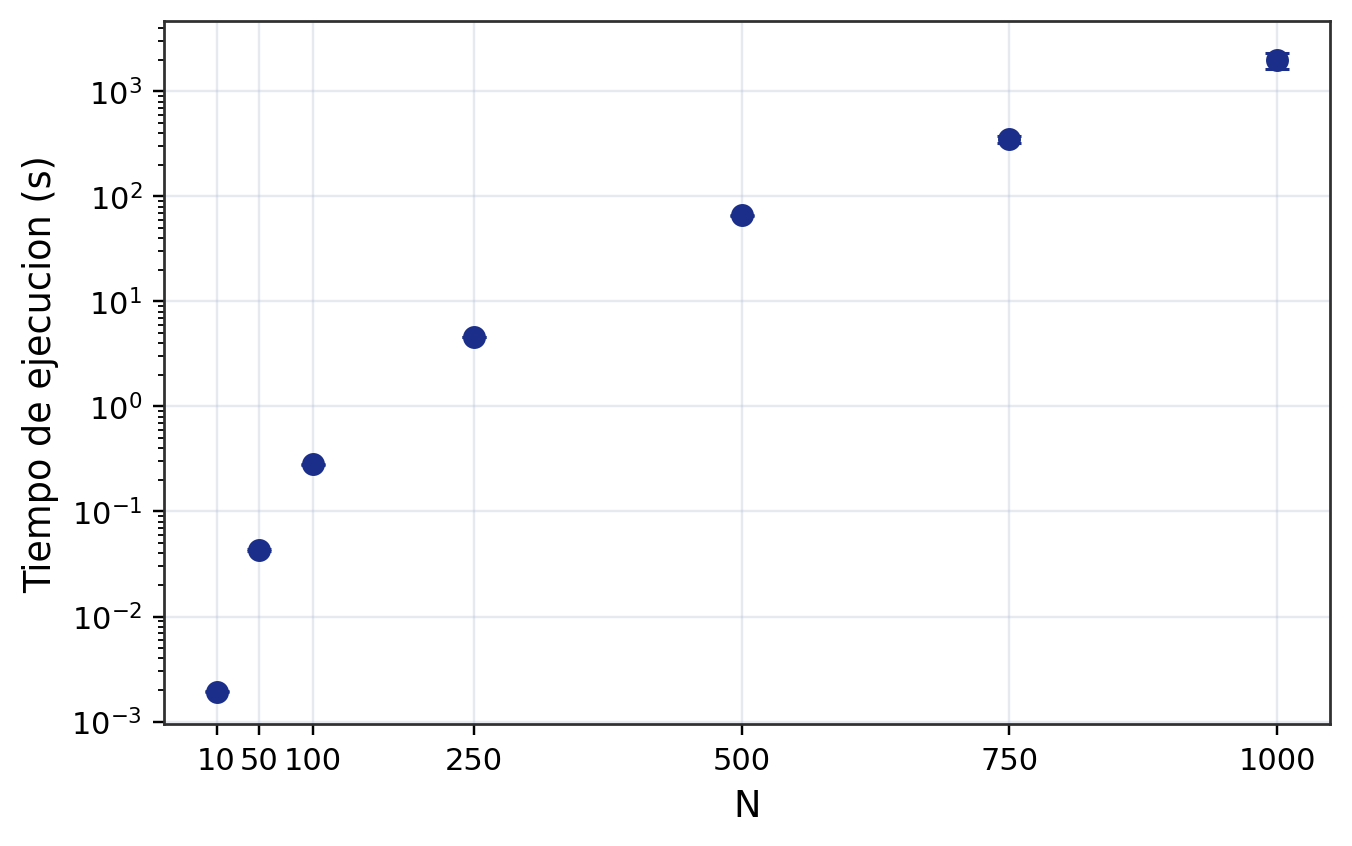
\includegraphics[width=\linewidth]{runtime_vs_n.png}

    \column{0.29\textwidth}
    \begin{block}{Lectura}
      \begin{itemize}
        \item 2 realizaciones por $N$
        \item Eje $Y$ logar\'itmico
        \item $N=250$: $4.61 \pm 0.02$ s
        \item $N=500$: $66.1 \pm 0.4$ s
        \item $N=1000$: $1980 \pm 340$ s
      \end{itemize}
    \end{block}
  \end{columns}
\end{frame}

\begin{frame}
  \frametitle{1.2 Evoluciones t\'ipicas de $C_{fc}(t)$}
  \begin{columns}[T,onlytextwidth]
    \column{0.49\textwidth}
    \centering
    {\small $N = 50$, realizaci\'on representativa\par}
    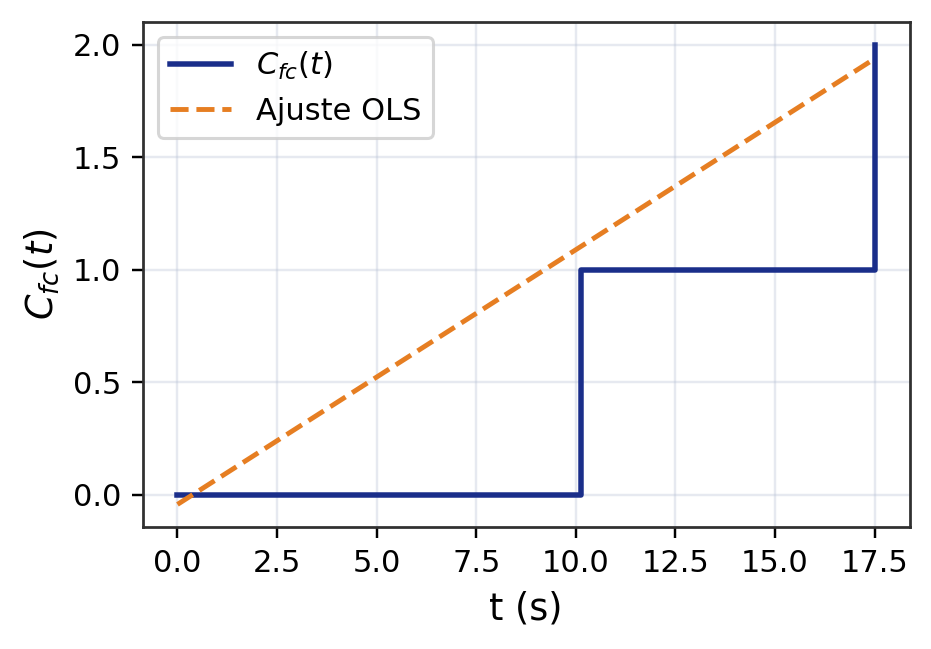
\includegraphics[width=\linewidth]{center_contacts_n_50_seed_100.png}

    \column{0.49\textwidth}
    \centering
    {\small $N = 1000$, realizaci\'on representativa\par}
    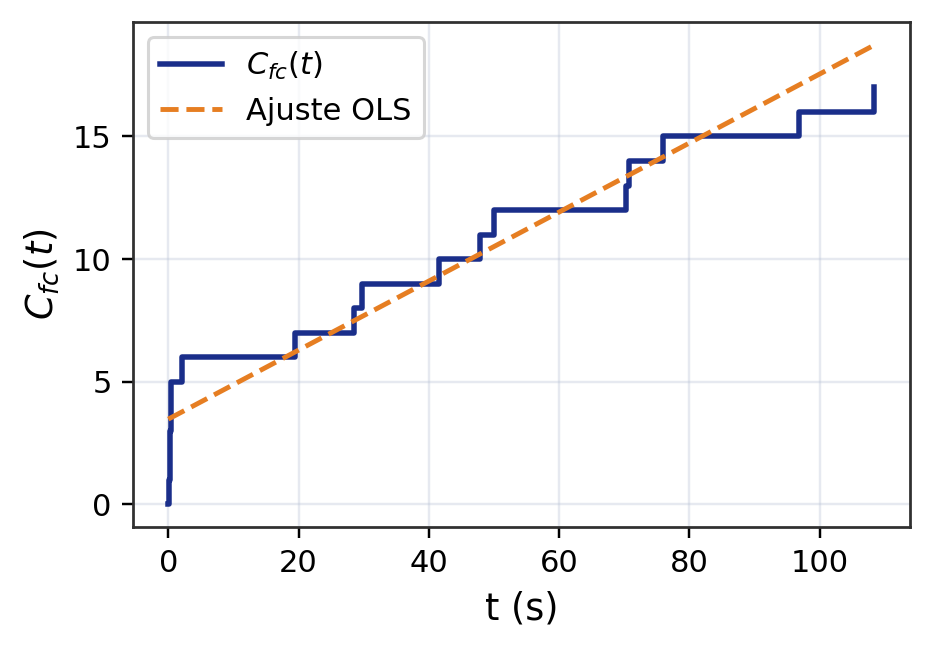
\includegraphics[width=\linewidth]{center_contacts_n_1000_seed_100.png}
  \end{columns}

  \vspace{0.14cm}
  {\small La pendiente del ajuste lineal define la tasa de escaneo de cada realizaci\'on. El barrido agregado de la diapositiva siguiente muestra que esa pendiente no var\'ia mon\'otonamente con $N$.}
\end{frame}

\begin{frame}
  \frametitle{1.2 Tasa de escaneo promedio}
  \begin{columns}[T,onlytextwidth]
    \column{0.71\textwidth}
    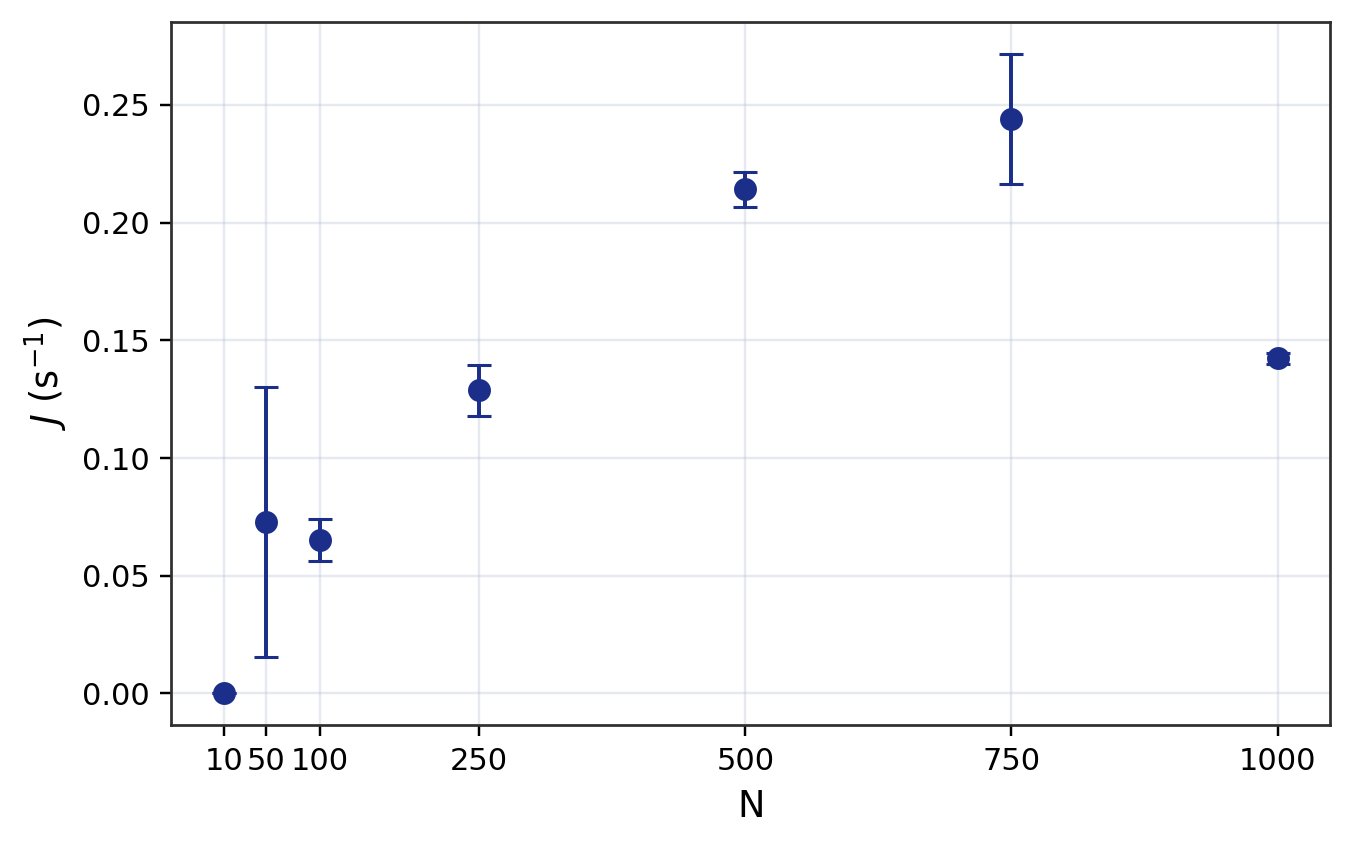
\includegraphics[width=\linewidth]{scanning_rate_vs_n.png}

    \column{0.29\textwidth}
    \begin{block}{Lectura}
      \begin{itemize}
        \item $J \approx 0$ para $N=10$
        \item M\'aximo medido en $N=750$
        \item $J(750)=0.244 \pm 0.028$
        \item $J(1000)=0.142 \pm 0.002$
      \end{itemize}
    \end{block}
  \end{columns}
\end{frame}

\begin{frame}
  \frametitle{1.3 Evoluciones t\'ipicas de $F_u(t)$}
  \begin{columns}[T,onlytextwidth]
    \column{0.49\textwidth}
    \centering
    {\small $N = 50$, realizaci\'on representativa\par}
    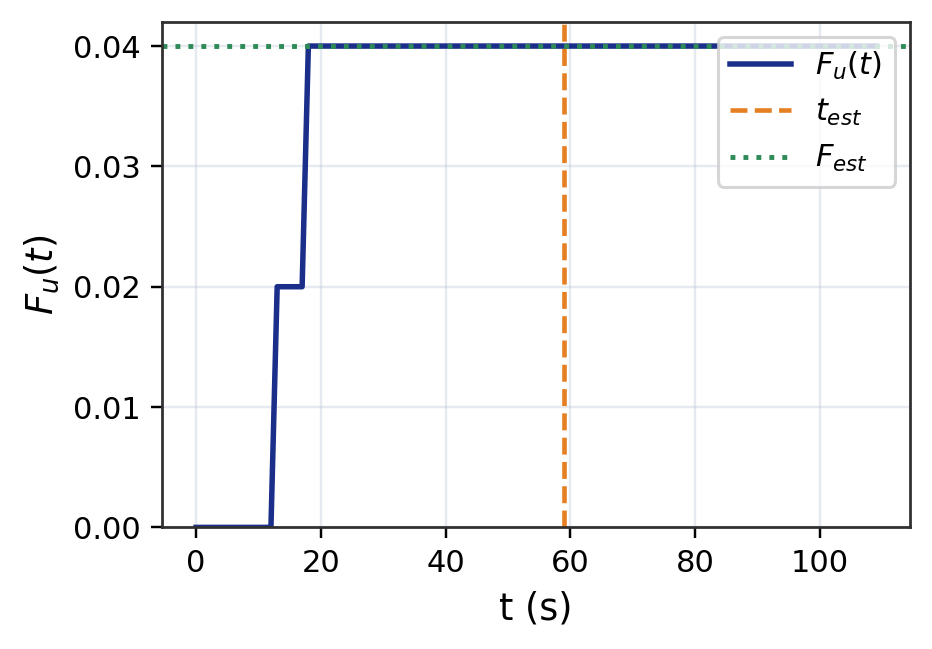
\includegraphics[width=\linewidth]{used_fraction_n_50_seed_100.png}

    \column{0.49\textwidth}
    \centering
    {\small $N = 1000$, realizaci\'on representativa\par}
    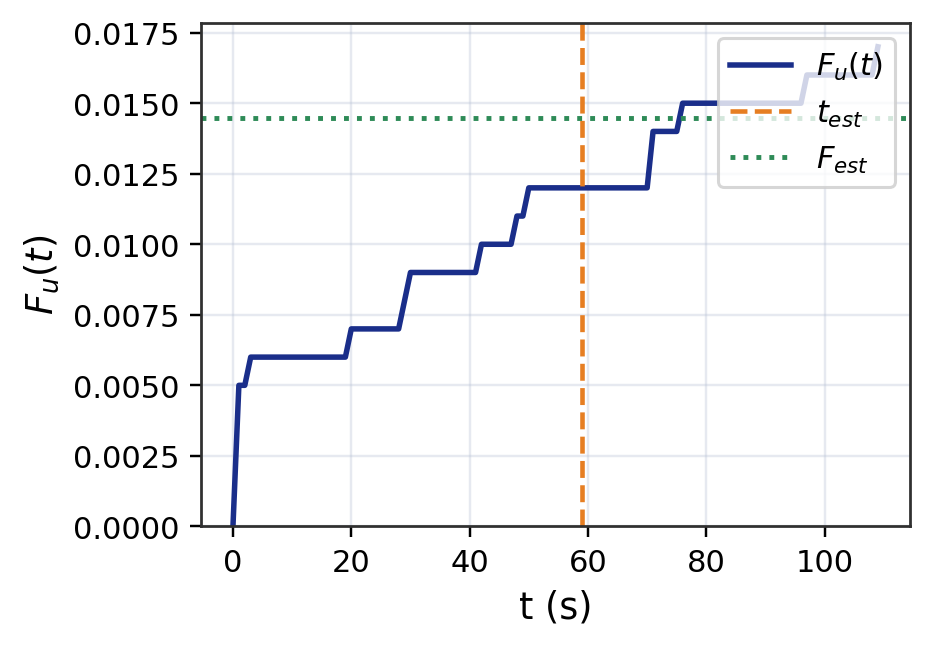
\includegraphics[width=\linewidth]{used_fraction_n_1000_seed_100.png}
  \end{columns}

  \vspace{0.14cm}
  {\small L\'inea punteada vertical: tiempo de estacionario $t_{est}$. L\'inea horizontal: promedio estacionario $F_{est}$.}
\end{frame}

\begin{frame}
  \frametitle{1.3 M\'etricas estacionarias}
  \begin{columns}[T,onlytextwidth]
    \column{0.49\textwidth}
    \centering
    {\small Tiempo al estacionario\par}
    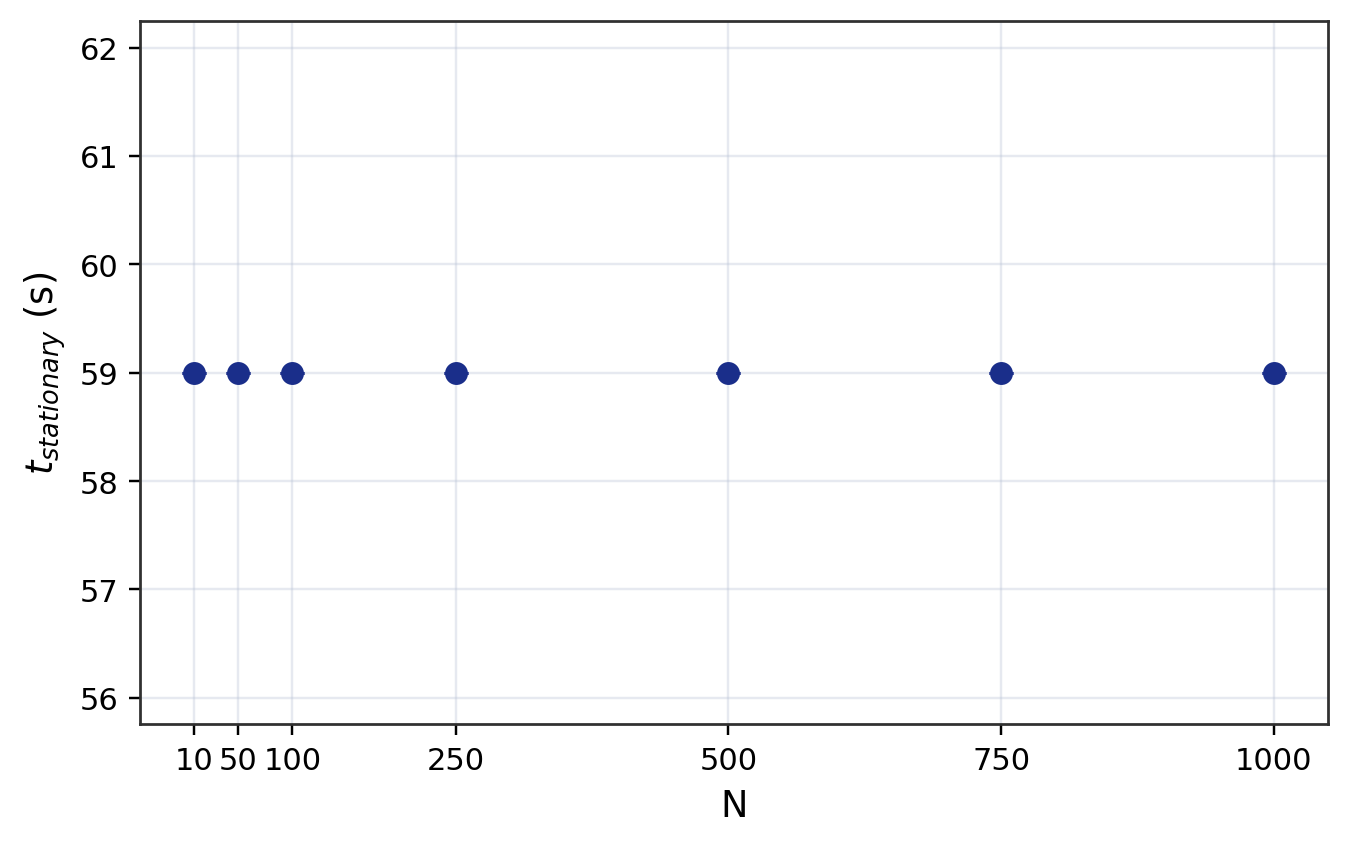
\includegraphics[width=\linewidth]{stationary_time_vs_n.png}

    \column{0.49\textwidth}
    \centering
    {\small Valor estacionario\par}
    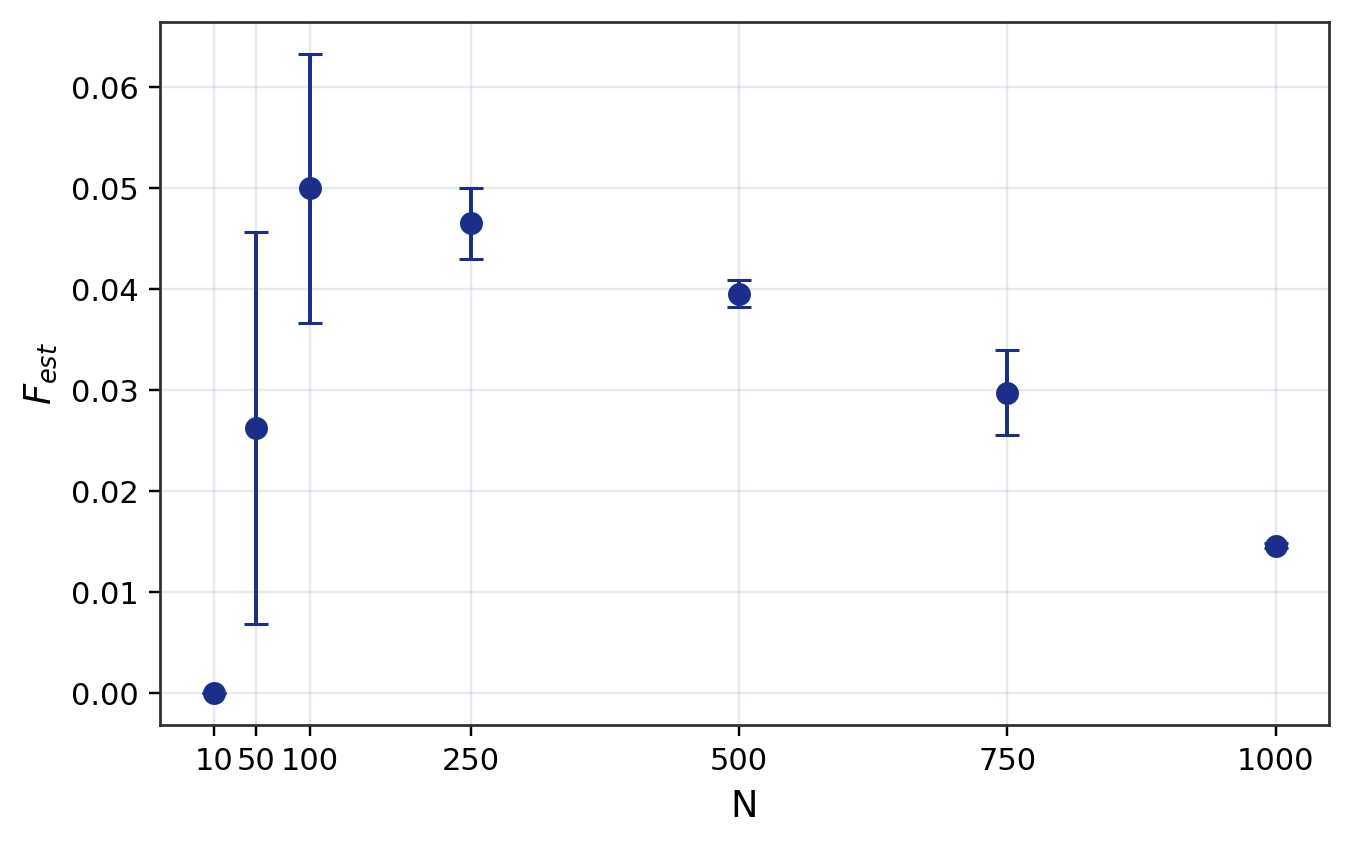
\includegraphics[width=\linewidth]{fest_vs_n.png}
  \end{columns}

  \vspace{0.1cm}
  {\small En esta base de datos todas las realizaciones alcanzan estacionario a los $59$ s. El valor m\'aximo de $F_{est}$ aparece en $N=100$ con $0.050 \pm 0.013$, y luego decrece hasta $0.0146 \pm 0.0002$ en $N=1000$.}
\end{frame}

\begin{frame}
  \frametitle{1.4 Perfil radial representativo}
  \begin{columns}[T,onlytextwidth]
    \column{0.74\textwidth}
    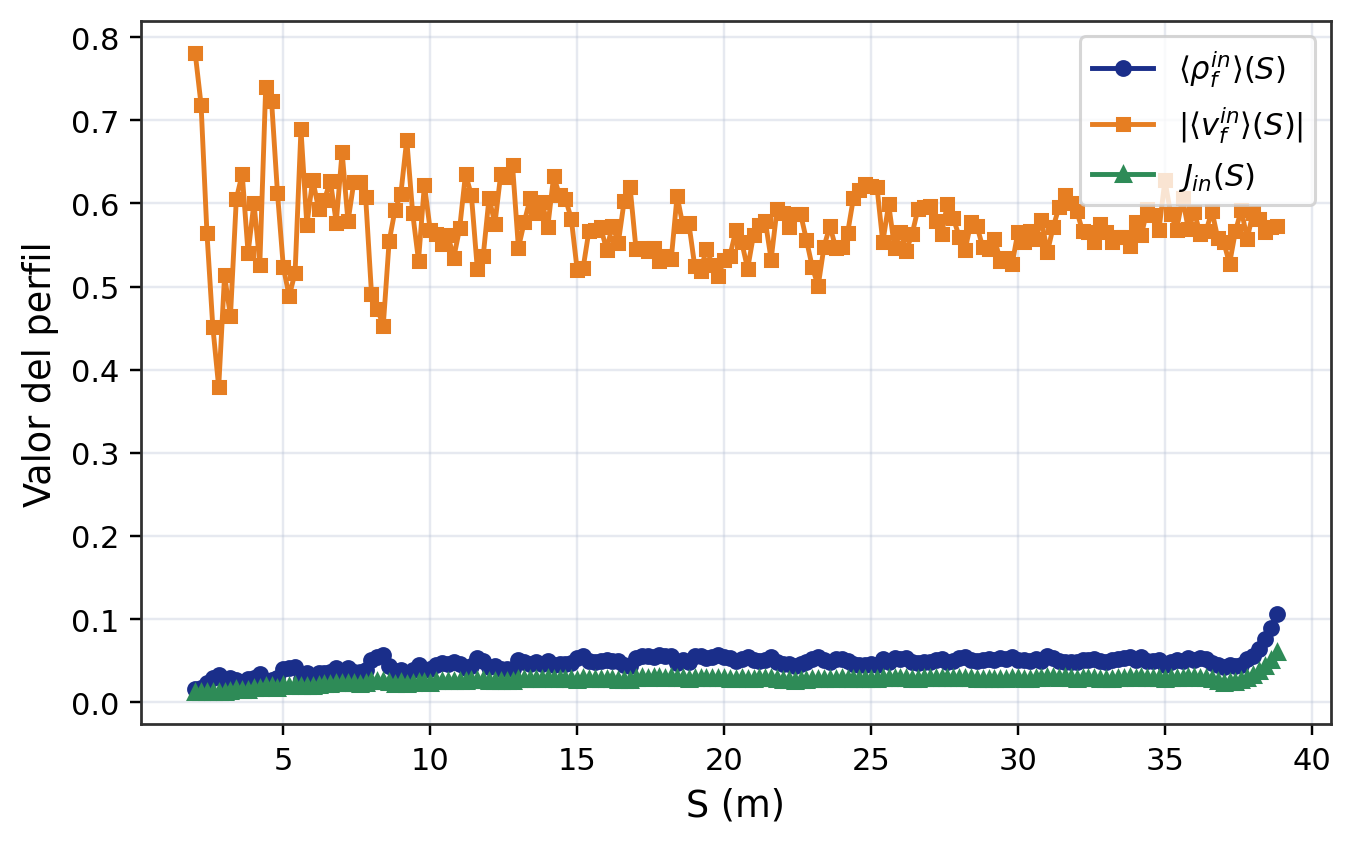
\includegraphics[width=\linewidth]{radial_profile_n_500.png}

    \column{0.26\textwidth}
    \begin{block}{Configuraci\'on}
      \begin{itemize}
        \item $N = 500$
        \item Promedio post-estacionario
        \item Solo part\'iculas frescas con $\bm{R}\cdot\bm{v}<0$
      \end{itemize}
    \end{block}
  \end{columns}
\end{frame}

\begin{frame}
  \frametitle{1.4 Capa cercana a $S \approx 2$}
  \centering
  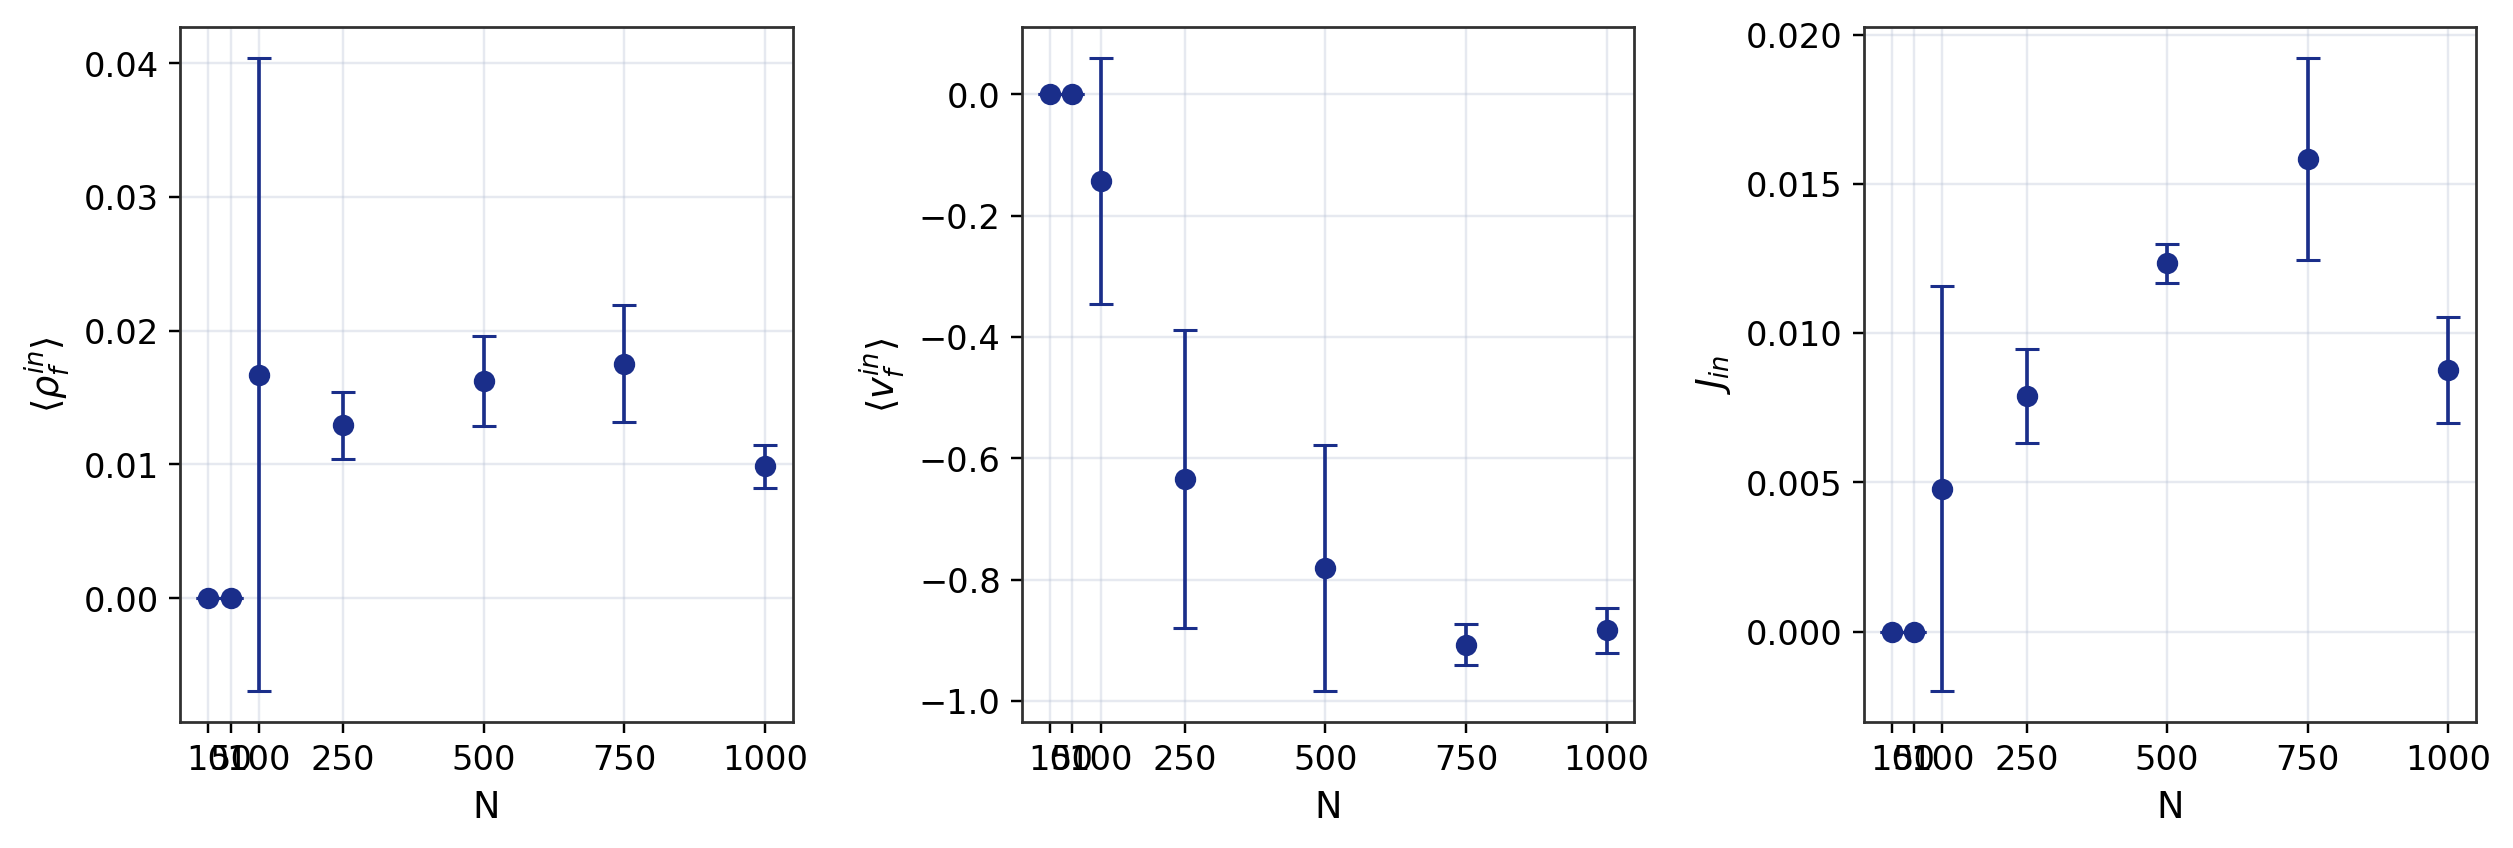
\includegraphics[width=0.96\linewidth]{near_shell_vs_n.png}

  \vspace{0.15cm}
  {\small Capa fija: $[2.0, 2.2)$. No se observa se\~nal para $N=10$ y $N=50$; el mayor flujo medido en esta grilla aparece en $N=750$.}
\end{frame}

\section{Conclusiones}
\sectiondivider{Conclusiones}

\begin{frame}
  \frametitle{Conclusiones generales}
  \small
  \begin{block}{Rendimiento computacional}
    \begin{itemize}
      \item El costo crece muy fuerte con $N$: pasar de $N=500$ a $N=1000$ lleva el tiempo medio de $66$ s a casi $1980$ s.
      \item La dispersi\'on de runtime tambi\'en aumenta en los reg\'imenes m\'as densos.
    \end{itemize}
  \end{block}

  \begin{block}{Observables globales}
    \begin{itemize}
      \item La tasa de escaneo no es mon\'otona en la grilla medida: crece hasta $N=750$ y luego cae en $N=1000$.
      \item Con este protocolo, todas las realizaciones alcanzan estacionario a $59$ s y la fracci\'on usada estacionaria disminuye para los $N$ m\'as grandes.
    \end{itemize}
  \end{block}
\end{frame}

\begin{frame}
  \frametitle{Conclusiones sobre la zona pr\'oxima al obst\'aculo}
  \footnotesize
  \begin{block}{Capa cercana a $S = 2$}
    \begin{itemize}
      \item Para $N$ chicos no hay se\~nal medible de part\'iculas frescas entrantes en la primera capa accesible.
      \item Desde $N=100$ aparecen densidad, velocidad normal y flujo distintos de cero.
      \item El m\'aximo observado en la capa $[2.0,2.2)$ ocurre en $N=750$ y luego cae en $N=1000$.
    \end{itemize}
  \end{block}

  \begin{block}{Alcance de estas conclusiones}
    \begin{itemize}
      \item Todas estas afirmaciones se apoyan en los resultados mostrados y en 2 realizaciones por valor de $N$.
      \item Tendencias m\'as finas exigir\'ian m\'as repeticiones o una grilla m\'as densa en $N$.
    \end{itemize}
  \end{block}
\end{frame}

\begin{frame}
  \begin{center}
    \vspace{1.8cm}
    {\LARGE Muchas gracias}

    \vspace{0.8cm}
    {\small Completar antes de entregar:\par}
    {\small \placeholder{NOMBRES, LEGAJOS, GRUPO Y LINKS DE ANIMACION}}
  \end{center}
\end{frame}

\end{document}
